% MplTplt - Yet another LaTeX template for Modern Physics Lab, PKU.
% Copyright (C) 2014 Huang Kangjing and contributors

% This work is completely rewritten basing on the work of Cao Chuanwu
% and Sun Sibai, with texts in the template originally coming from the
% Modren Phys. Lab.

% This file is released under the MIT license.
%
% Permission is hereby granted, free of charge, to any person obtaining a copy
% of this software and associated documentation files (the "Software"), to deal
% in the Software without restriction, including without limitation the rights
% to use, copy, modify, merge, publish, distribute, sublicense, and/or sell
% copies of the Software, and to permit persons to whom the Software is
% furnished to do so, subject to the following conditions:
% 
% The above copyright notice and this permission notice shall be included in
% all copies or substantial portions of the Software.
% 
% THE SOFTWARE IS PROVIDED "AS IS", WITHOUT WARRANTY OF ANY KIND, EXPRESS OR
% IMPLIED, INCLUDING BUT NOT LIMITED TO THE WARRANTIES OF MERCHANTABILITY,
% FITNESS FOR A PARTICULAR PURPOSE AND NONINFRINGEMENT. IN NO EVENT SHALL THE
% AUTHORS OR COPYRIGHT HOLDERS BE LIABLE FOR ANY CLAIM, DAMAGES OR OTHER
% LIABILITY, WHETHER IN AN ACTION OF CONTRACT, TORT OR OTHERWISE, ARISING FROM,
% OUT OF OR IN CONNECTION WITH THE SOFTWARE OR THE USE OR OTHER DEALINGS IN
% THE SOFTWARE.
%

% This template depends on the "revtex4.1" package from APS Journals
% <http://publish.aps.org/revtex/revtex-faq>, and the Chinese handling
% is done with XeLaTeX engine and package "xeCJK". Please ensure these
% packages are available in your chosen Tex software distribution.

% Document created using this template should be compiled with XeLaTeX
% engines rather than plain LaTeX or plain TeX engines.

% The non-ASCII texts of this template is encoded in UTF-8 encoding.
% Please note that XeLaTeX only accepts UTF-8 encoded documents, so
% set your editor to use UTF-8 while creating documents with this template.

% Recommended TeX software distribution to use with this template is
% Tex Live developed by the TeX User Group (TUG), please visit the home
% page of the distribution <https://www.tug.org/texlive/> for further details.

% NOTE THAT IMPORTANT INSTRUCTIONS HAS BEEN WRITTEN AS UPPERCASE COMMENTS
% IN THE TEXT, PLEASE READ THEM CAREFULLY AND FOLLOW THEM TO MAKE THE
% TEMPLATE WORK!

% Any further contributions to the template is welcome, please send
% pull requests through github or send mail to maintainer.

% For any other questions, please do not hesitate to contact maintainer.

% Current maintainer:
% Huang Kangjing <huangkangjing@gmail.com>

% Contributors:
% Sun Sibai <niasw@pku.edu.cn>
% Cao Chuanwu <>
% Huang Kangjing <huangkangjing@gmail.com>


\documentclass[aps,pre,12pt,preprint,onecolumn,showpacs,showkeys]{revtex4-1}

% Setting up Chinese handling.
\usepackage{fontspec,xeCJK}

% Setting up fonts.
% PLEASE MODIFY ALL THESE FONT NAMES ACCORDING TO YOUR FONT
% INSTALLATION AND PERFERENCE.

% Setting up main fonts and mono fonts.
\setmainfont{Liberation Serif}
\setmonofont{Liberation Mono}
% SimSun is required font for the main body of the text.
\setCJKmainfont[AutoFakeBold=5,AutoFakeSlant]{SimSun}
\setCJKmonofont[AutoFakeBold=2,AutoFakeSlant]{SimHei}

% Setting up alternative font families.
% Note that these three fonts below are required fonts in document
% title, section headings and figure captions.
\newCJKfontfamily\heiti[AutoFakeBold=2,AutoFakeSlant]{SimHei}
\newCJKfontfamily\fangsong[AutoFakeBold=5,AutoFakeSlant]{FangSong}
\newCJKfontfamily\kaiti[AutoFakeBold=5,AutoFakeSlant]{KaiTi}

% Setting up paragraph indent.
\parindent 2em

% Setting up macros for Chinese-style font size setting.
\newcommand{\fseight}{\fontsize{5.02}{6.02}\selectfont}
\newcommand{\fsseven}{\fontsize{5.52}{6.62}\selectfont}
\newcommand{\fsssix}{\fontsize{6.52}{7.83}\selectfont}
\newcommand{\fssix}{\fontsize{7.53}{9.03}\selectfont}
\newcommand{\fssfive}{\fontsize{9.03}{10.84}\selectfont}
\newcommand{\fsfive}{\fontsize{10.54}{12.65}\selectfont}
\newcommand{\fssfour}{\fontsize{12.05}{14.45}\selectfont}
\newcommand{\fsfour}{\fontsize{14.05}{16.86}\selectfont}
\newcommand{\fssthree}{\fontsize{15.06}{18.07}\selectfont}
\newcommand{\fsthree}{\fontsize{16.06}{19.27}\selectfont}
\newcommand{\fsstwo}{\fontsize{18.07}{21.68}\selectfont}
\newcommand{\fstwo}{\fontsize{22.08}{26.50}\selectfont}
\newcommand{\fssone}{\fontsize{24.09}{28.91}\selectfont}
\newcommand{\fsone}{\fontsize{26.10}{31.32}\selectfont}
\newcommand{\fsszero}{\fontsize{36.14}{43.36}\selectfont}
\newcommand{\fszero}{\fontsize{42.16}{50.59}\selectfont}

% Replace words to Chinese corespondence.
\renewcommand\appendixname{附录}
\renewcommand\abstractname{}
\renewcommand\tablename{表}
\renewcommand\figurename{图}

% Replace words in revtex4-1 to Chinese corespondence.
\makeatletter
\def\@pacs@name{\heiti\fssfour \textbf{PACS码:}\normalfont}
\def\@keys@name{\heiti\fssfour \textbf{关键词:}\normalfont}
\def\Dated@name{日期:}
\def\Received@name{\fssfive 接收 }
\def\Revised@name{\fssfive 修订 }
\def\Accepted@name{\fssfive 采纳 }
\def\Published@name{\fssfive 发表 }
\makeatother

% Change label style of enumerate.
\renewcommand{\labelenumi}{\alph{enumi}.}

% Setting up geometry.
\usepackage{geometry}
\geometry{top=2.54cm,bottom=2.54cm,left=3cm,right=3cm}

% Setting up line space.
\usepackage{setspace}
\linespread{1.6}

% Setting up hyperreferences.
\usepackage{hyperref}
\hypersetup{colorlinks=true}

% Setting up styles for section headings.
\usepackage{titlesec}
\titleformat*{\section}{\bf\fangsong\fsfour}
\titleformat*{\subsection}{\bf\fangsong}

% Loading packages for image handling.
\usepackage{subfig}
\usepackage{graphicx,psfrag,epsfig}

% Setting up caption styles.
\usepackage{caption}
\DeclareCaptionFont{kaiti}{\kaiti}
\DeclareCaptionFont{bfheiti}{\bf\heiti}
\captionsetup{font=small,format=plain,labelfont=bfheiti,%
  textfont=kaiti,justification=raggedright,%
  singlelinecheck=false}

% Loading packages for math typings.
\usepackage{amsmath,amsfonts,amssymb,amsthm,bm,upgreek}
\usepackage[mathscr]{eucal}
\usepackage{siunitx}
\usepackage{listings,color}
\lstset{%
    breaklines=true,
    basicstyle=\fontspec{Liberation Mono}\footnotesize,
    commentstyle=\fontspec{Liberation Mono}\it\color{green},
    showspaces=false,
    stringstyle=\fontspec{Liberation Mono}\bf,
    numbers=left,
    numberstyle=\fontspec{Liberation Mono}\tiny,
    keywordstyle=\fontspec{Liberation Mono}\bf\color{blue},
    title=\lstname,
    frame=L}

\begin{document}

% Title and author info.
\title{\bf\heiti\fsthree 晶体的电光效应及其应用\vspace{15mm}}
\author{\fangsong\fsfour 黄康靖\vspace{2mm}}
\affiliation{\normalfont\fssfour 2012级~~~~学号:{masked student id}\vspace{2mm}}
\date{March 27, 2015}
\keywords{双折射,磷酸二氘钾,电光效应,光学调制器}
\email{huangkangjing@gmail.com}

% Abstract.
\begin{abstract}
  \vspace{10mm}
  \begin{spacing}{1.5}
    \fssfour
    本实验首先通过对于磷酸二氘钾晶体的电光效应的研究,探究了电光效应的基本原理,测明了
    磷酸二氘钾晶体的半波电压与电光系数.并随后使用测得的晶体参数和晶体本身,利用相
    位补偿法,测得了云母片晶体样本的折射率差,从而探究了晶体电光效应的相关应用.
  \end{spacing}
\end{abstract}

% The main body of the document goes from here.
\maketitle
\fssfour
\section{引言}

当光介质(比如晶体或者液体)加上电场之后,其折射率发生变化的现象成为电光效应.电光效
应是介质在外加电场下的极化现象中的非线性效应的体现.电场与介质折射率之间的变化关
系可以用下式表示:
\begin{equation}
    n = n^0 + a E_0 + b E_0^2 + \dots
\end{equation}
其中$a,b$为常数,$n^0$为无电场作用时的折射率,由一次项$aE_0$引起的折射率变化称为一
次电光效应,也称作线性电光效应或者泡克耳斯效应,是1893年由泡克耳斯发现的,它只存在
于没有对称中心的晶体中,总共只有20多种晶体类型.而由二次项$bE_0^2$引起的折射率变化
被称为二次电光效应,也称为平方电光效应或者克尔效应,它存在于所有的电介质中,数值上
远远小于一次电光效应,因此通常不予考虑.

电光效应在科学研究与工程技术中有许多重要应用,如可以制成光相位调制器,光开关,光滤
波器,光衰减器.特别是在激光出现以后,电光晶体被广泛应用在激光通讯,激光测距,激光显
示,光学数据处理等方面.现在电光效应的测量已经成为研究电光晶体,液晶,功能有机分子与
聚合物的一种重要手段.

本实验研究了KD*P(KD$_2$PO$_4$,磷酸二氘钾)晶体的一次电光效应.本实验分别采用了三种
不同方法测量晶体的半波电压值,从而得出电光系数.最后用电光晶体作为相位补偿器,测量
出云母等双折射样品的微小相位差.\cite{Book}

\section{原理}

\subsection{一次电光效应的一般描述}

光在各向异性晶体中传播时,因光的传播方向或者电矢量的振动方向不同,光的折射率也不同
,这一区别通常采用折射率椭球来描述.在主轴坐标系中,折射率椭球方程为:
\begin{equation}
    \frac{x^2}{n_1^2} + \frac{y^2}{n_2^2} +  \frac{z^2}{n_3^2} = 1
\end{equation}

当晶体加上电场之后,折射率椭球的形状,大小,方位都发生变化,椭球方程变成
\begin{equation}
    \frac{x^2}{n_{11}^2} + \frac{y^2}{n_{22}^2} + \frac{z^2}{n_{33}^2} +
    \frac{2}{n_{23}^2}yz + \frac{2}{n_{13}^2}xz + \frac{2}{n_{12}^2}xy = 1
\end{equation}
只考虑一次电光效应的情况下,电场对折射率椭球的影响可以用以下矩阵形式表示:
\begin{equation}
    \begin{pmatrix}
        \frac{1}{n_{11}^2} - \frac{1}{n_1^2} \\
        \frac{1}{n_{22}^2} - \frac{1}{n_2^2} \\
        \frac{1}{n_{33}^2} - \frac{1}{n_3^2} \\
        \frac{1}{n_{23}^2} \\
        \frac{1}{n_{13}^2} \\
        \frac{1}{n_{12}^2}
    \end{pmatrix}
    = \begin{pmatrix}
        r_{11} & r_{12}  & r_{13} \\
        r_{21} & r_{22}  & r_{23} \\
        r_{31} & r_{32}  & r_{33} \\
        r_{41} & r_{42}  & r_{43} \\
        r_{51} & r_{52}  & r_{53} \\
        r_{61} & r_{62}  & r_{63} 
    \end{pmatrix}
    \begin{pmatrix}
        E_x \\
        E_y \\
        E_z
    \end{pmatrix}
\end{equation}\cite{Book}

\subsection{磷酸二氘钾类型晶体的纵向电光效应}

KD*P晶体是一种人工生长的晶体,与他同类型的还有KDP(磷酸二氢钾)和ADP(磷酸二氢铵),它
们属于四方晶系.

KD*P为负单轴晶体,折射率椭球为旋转椭球,表达式为:
\begin{equation}
    \frac{x^2 + y^2}{n_o^2} + \frac{z^2}{n_e^2} = 1
\end{equation}
式中$n_o$与$n_e$分别为单轴晶体的寻常光折射率与非寻常光折射率.

由晶体的对称性与前述的电光效应的普遍表达形式,我们可以得到加上电场之后,折射率椭球
方程应当成为
\begin{equation}
    \frac{x^2 + y^2}{n_o^2} + \frac{z^2}{n_e^2} + 2r_{41}(E_xyz + E_yxz) +
    2r_{63}E_zxy = 1
\end{equation}
即加上电场后,折射率椭球由旋转椭球变为一般的椭球.

如果只在KD*P晶体的光轴z方向上加电场,则折射率椭球式成为
\begin{equation}
    \frac{x^2 + y^2}{n_o^2} + \frac{z^2}{n_e^2} + 2r_{63}E_zxy = 1
\end{equation}

为了求出加电场后朱折射率的变化,作如下坐标变换
\begin{equation}
    \begin{cases}
        x = x'\cos{\frac{\pi}{4}} - y'\sin{\frac{\pi}{4}} \\
        y = x'\sin{\frac{\pi}{4}} + y'\cos{\frac{\pi}{4}} \\
        z = z'
    \end{cases}
\end{equation}
可得折射率椭球方程为
\begin{equation}
    \frac{x'^2}{n_{x'}^2} + \frac{y'^2}{n_{y'}^2} + \frac{z'^2}{n_{z'}^2} = 1
\end{equation}
并且
\begin{equation}
    \begin{cases}
        n_{x'} = n_o(1 + n_o^2r_{63}E_z)^{-1/2} \\
        n_{y'} = n_o(1 - n_o^2r_{63}E_z)^{-1/2} \\
        n_{z'} = n_z
    \end{cases}
\end{equation}
当折射率的变化很小时,有
\begin{equation}
    \begin{cases}
        n_{x'} \approx n_o - \frac{n_o^3}{2}r_{63}E_z \\
        n_{y'} \approx n_o + \frac{n_o^3}{2}r_{63}E_z \\
        n_{z'} = n_z
    \end{cases}
\end{equation}

当光束沿着晶体光轴$z$方向传播时,沿着$x'$轴振动的光波和沿着$y'$轴振动的光波,由于它们
的折射率不同,经过长度为$l$的晶体后,产生的相位差为
\begin{equation}
    \Phi = \frac{2\pi}{\lambda}(n_{y'} - n_{x'})l =
    \frac{2\pi}{\lambda}n_o^3r_{63}E_zl = \frac{2\pi}{\lambda}n_o^3r_{63}V_D
\end{equation}
这里$V_D$是加在晶体$z$方向的直流电压,称为半波电压,其表达式为
\begin{equation}
    V_{\pi} = \frac{\lambda}{2n_o^3r_{63}}
\end{equation}
由此可得电光效应的电光系数的测量原理式
\begin{equation}
    r_{63} = \frac{\lambda}{2n_o^3V_{\pi}}
\end{equation}\cite{Book}

\section{实验}

实验的装置示意图如图~\ref{fig:ins}所示

\begin{figure}[htbp]
    \centering
    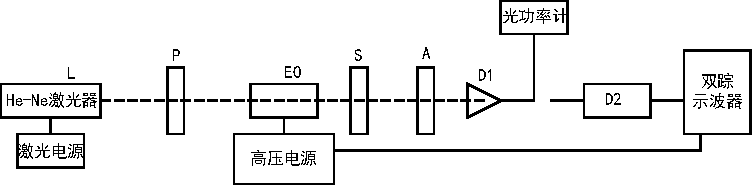
\includegraphics[width=\textwidth]{drawing.pdf}
    \caption{\label{fig:ins}%
        此图为实验装置的示意图.实验装置基本上由氦氖激光器,起偏器,电光晶体,测量样
        品,检偏器和探测器这几部分组成.其中探测器部分在实验的不同阶段分别使用了光
        功率计与光电集成接受装置.}
\end{figure}

实验使用的激光器是内腔型氦氖气体激光器,使用JDW-3型激光电源供电.

如前文所述,实验中使用的电光晶体是KD*P(磷酸二氘钾)晶体.\cite{Book}

实验分为三部分进行:

\begin{enumerate}
    \item 在这一部分中,首先A与P的偏振状态被调节成相互垂直着,并且分别与电光晶体的$x$主轴和$y$主
        轴相互平行的状态, 测量了电光晶体上加上的电压与输出的光强之间的关系.
        随后,P被调节为与A的偏振状态平行的状态,测量了电光晶体上加上的电压与输出的
        光强之间的关系.
    \item 在这一部分中,如同在上一个部分中一样,A与P的偏振状态先后被调节成分别与电
        光晶体的两个主轴平行与一同和晶体的一个主轴平行的状态.实验在这一部分中采
        用光电探测器进行测量,并且使用交流信号源,在高压直流电压的基础上,在电光晶
        体上加上了一个交变电压.

        数学分析可以得出,当直流电压在V-I曲线最高和最低值的中部时,输出的光强在这
        一条件下将以交变电源的频率交变变化;而当直流电压在V-I曲线的最高值和最低值
        点时,输出的光强的交变频率将会出现二倍频现象.这是测量V-I曲线最值点的精确
        度较高的有效方法.

        在这一部分中,实验使用了上述的方法,在上述的两种条件中分别测量了V-I曲线的最高
        点位置.
    \item 在这一部分中,样品片S被插入到了光路中,并且其光轴被调节为与电光晶体的光
        轴相互平行.
        随后,使用了与第二部分中相同的方法与条件,分别测量了两种条件下V-I曲线最高
        值点的位置.这样,若样品的相位差记为$\Phi_S$,两种情况下电光晶体的加的电压
        分别为$V_D$和$V'_D$,那么我们分别可以有
        \begin{equation}
            \Phi_S = -\frac{\pi V_D}{V_{\pi}}
        \end{equation}
        和
        \begin{equation}
            \Phi_S = \pi - \frac{\pi V'_D}{V_{\pi}}
        \end{equation}
        从而可以测得样品的$\Phi_S$,结合样品的厚度就可以算出样品的$\Delta n$.并且
        可以测得电光晶体的半波电压:
        \begin{equation}
            V'_D - V_D = V_{\pi}
        \end{equation}
\end{enumerate}

\section{实验结果及分析讨论}

\begin{enumerate}
    \item
        对于第一部分的实验,测得的V-I特性曲线如图~\ref{fig:plot1}和图
        ~\ref{fig:plot2}所示

        根据曲线,我们可以得到粗测的电光晶体半波长度为
        \begin{equation}
            V_{\pi} = \SI{1341}{V}
        \end{equation}

\begin{figure}[htbp]
    \centering
    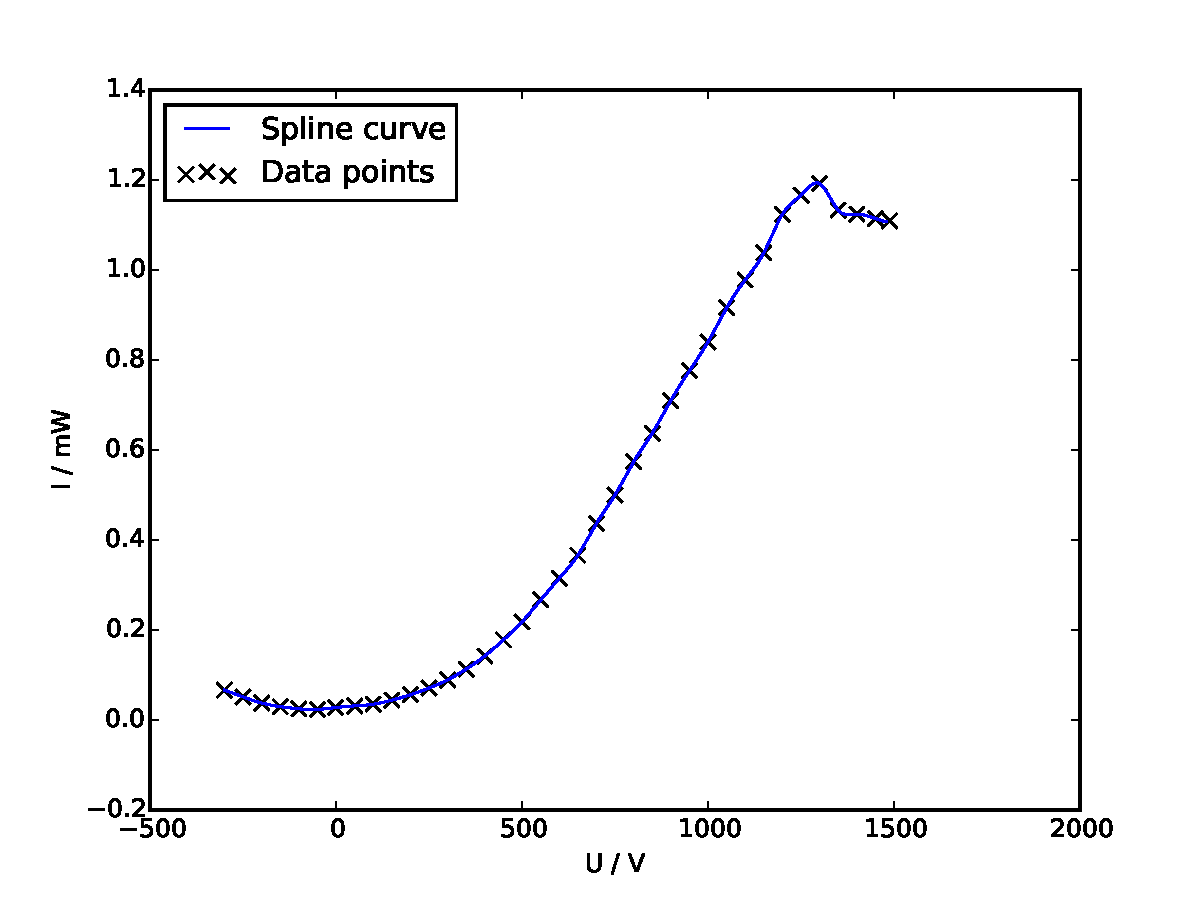
\includegraphics[width=\textwidth]{figure_1.pdf}
    \caption{\label{fig:plot1}%
        当A与P的偏振方向分别与电光晶体的两个主轴分别平行时测得的电光晶体电压与输
        出光强之间的关系曲线;拟合曲线为数据点按照三阶分段样条插值算法得到}
\end{figure}

\begin{figure}[htbp]
    \centering
    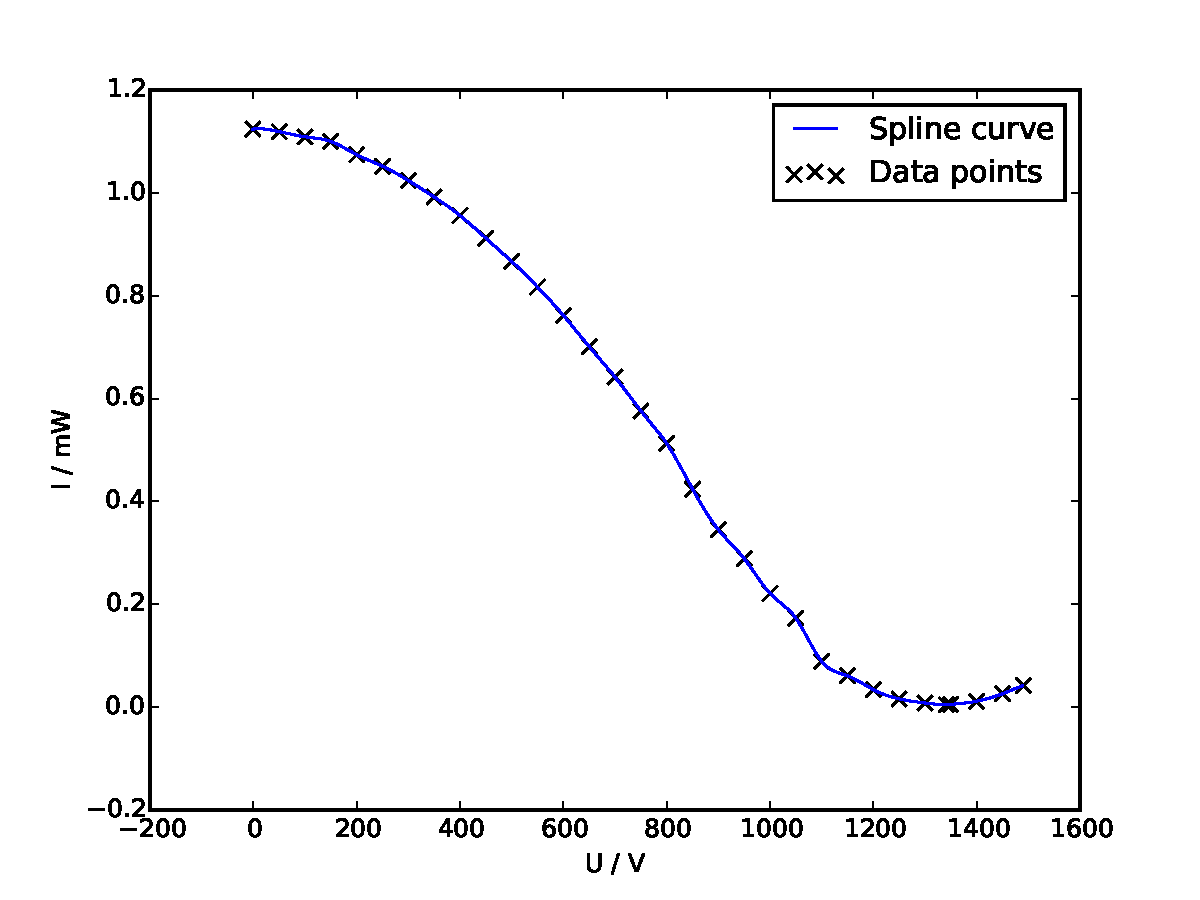
\includegraphics[width=\textwidth]{figure_2.pdf}
    \caption{\label{fig:plot2}%
        当A与P的偏振方向一同与电光晶体的某个主轴一致平行时测得的电光晶体电压与输
        出光强之间的关曲线;拟合曲线为数据点按照三阶分段样条插值算法得到}
\end{figure}

\item
    对于第二部分的实验,根据在两种不同条件下的输出光强极值位置,我们测得了晶体半波
    电压应为
    \begin{equation}
        V_{\pi} = \SI{1424}{V}
    \end{equation}
    并且,由每块晶体长度为$l = \SI{1.5}{cm}$,激光波长为$\lambda = \SI{632.8}{nm}$的实验室数据,我们计算得出晶体的电光系
    数为
    \begin{equation}
        r_{63} = \SI{1.62e-11}{V^{-1}m^{-1}}
    \end{equation}

\item
    对于第三部分的实验,我们通过补偿法,测得了云母样品的折射率差应当为
    \begin{equation}
        \Delta n = \num{2.64e-6}
    \end{equation}

\end{enumerate}

\section{结论}

本次实验研究并考察了KD*P晶体的电光效应,先测量了搭建的光学系统的V-I响应曲线,测得
了该晶体的半波电压,并且在此基础上测得了晶体的电光系数.

随后,本实验利用已测得的晶体的电光系数,采用补偿法进行测量,成功地完成了对云母晶体样本
片的折射率插值测量.

本次测量中,我们采用了调整起偏器P而不是检偏器A的做法.理论上来说,这一做法可能会给
系统引入误差,因为激光发射的入射光并不一定是无偏振光或者圆偏振光,从而调节起偏器可
能改变入射到系统中的光强度.然而,从实验的结果来看,结果并没有和标准值有太大偏离,从
而证明了这一引入的误差是微弱的.


\section{致谢}

感谢蒋莹莹老师在实验中认真而细致的指导.

感谢同组的冯一阳同学在实验中仔细而周到的协助.

\begin{thebibliography}{}
\bibitem{Book} 吴思成,王祖铨~2010 近代物理实验(第三版)(北京:高等教
育出版社)第165页.  %实验书
\end{thebibliography}

\clearpage
\appendix
\section{思考题}

\begin{enumerate}
    \item
        本实验先后采用了直接测量极值,使用倍频法测量极值,和加入样品用补偿法测量半
        波电压的方法.三个方法一个比一个精确,但是操作一个比一个麻烦.
    \item
        主要由光电晶体和配套的电压源组成.它的作用是可以可调整地控制通过它的光的
        偏振态
    \item
        这将导致在后面测量半波电压的步骤中难以调节到输出光强的最低点,从而引入半
        波电压的测
        量误差.
    \item
        因为这一方法对于判断极值点的位置最为精确,可以有效控制测量误差.
\end{enumerate}

\section{代码}

本实验的所有数据处理和绘图使用python语言完成.具体的处理使用了python的numpy,scipy
和matplotlib这数个开放源代码库套件.

相关的处理代码附在文后

\lstinputlisting[language=python]{plot1.py}
\lstinputlisting[language=python]{plot2.py}

\end{document}
